

\documentclass[11pt,a4paper]{article}
\usepackage{acl2015}
\usepackage{times}
\usepackage{latexsym}
% \setlength\titlebox{5cm}    % Expanding the titlebox

%%% Custom additions %%%
% \usepackage{hyperref}
\usepackage{url}
\usepackage[leqno, fleqn]{amsmath}
\usepackage{amssymb}
\usepackage{qtree}
\usepackage{graphicx}
\usepackage{booktabs}
\usepackage{multirow}
\usepackage{colortbl}
\usepackage{caption}
\usepackage{subcaption}
\usepackage{color}
\usepackage{xcolor}
\usepackage{tikz}
\usepackage{ifthen}
\usepackage{framed}



\def\entailment{\textit{entailment}}
\def\unknown{\textit{unknown}}
\def\contradiction{\textit{contradiction}}
\def\hypothesis{hypothesis}
\def\premise{premise}


\usepackage{color}
\newcommand{\hl}[2]{\colorbox{#2}{#1}}
\newcommand{\hly}[1]{\hl{yellow}{#1}}
\def\todo#1{\hl{{\bf TODO:} #1}{yellow}}
\def\needcite{\hl{{$^{\tt\small[citation\ needed]}$}}{blue}}
\def\needfig{\hl{Figure X}{green}}
\def\needtab{\hl{Table Y}{green}}

\newcommand\fig[1]{\begin{center} \includegraphics{#1} \end{center}}
\newcommand\Fig[4]{\begin{figure}[tb] \begin{center} \includegraphics[scale=#2]{#1} \end{center} \caption{\label{fig:#3} #4} \end{figure}}
\newcommand\FigTop[4]{\begin{figure}[t] \begin{center} \includegraphics[scale=#2]{#1} \end{center} \caption{\label{fig:#3} #4} \end{figure}}
\newcommand\FigStar[4]{\begin{figure*}[tb] \begin{center} \includegraphics[scale=#2]{#1} \end{center} \caption{\label{fig:#3} #4} \end{figure*}}

\newcommand\refeqn[1]{(\ref{eqn:#1})}
\newcommand\refeqns[2]{(\ref{eqn:#1}) and (\ref{eqn:#2})}
\newcommand\refchp[1]{Chapter~\ref{chp:#1}}
\newcommand\refsec[1]{Section~\ref{sec:#1}}
\newcommand\refsecs[2]{Sections~\ref{sec:#1} and~\ref{sec:#2}}

\newcommand\Reffig[1]{Figure~\ref{#1}}
\newcommand\Reffigs[2]{Figures~\ref{#1} and~\ref{#2}}
\newcommand\Reffigss[3]{Figures~\ref{#1},~\ref{#2}, and~\ref{#3}}
\newcommand\Reffigsss[4]{Figures~\ref{#1},~\ref{#2},~\ref{#3}, and~\ref{#4}}

\newcommand\reffig[1]{Figure~\ref{#1}}
\newcommand\reffigs[2]{Figures~\ref{#1} and~\ref{#2}}
\newcommand\reffigss[3]{Figures~\ref{#1},~\ref{#2}, and~\ref{#3}}
\newcommand\reffigsss[4]{Figures~\ref{#1},~\ref{#2},~\ref{#3}, and~\ref{#4}}

\newcommand\reftab[1]{Table~\ref{#1}}
\newcommand\Reftab[1]{Table~\ref{#1}}
\newcommand\reftabs[2]{Tables~\ref{#1} and \ref{#2}}


\newcommand\refapp[1]{Appendix~\ref{sec:#1}}
\newcommand\refthm[1]{Theorem~\ref{thm:#1}}
\newcommand\refthms[2]{Theorems~\ref{thm:#1} and~\ref{thm:#2}}
\newcommand\reflem[1]{Lemma~\ref{lem:#1}}
\newcommand\reflems[2]{Lemmas~\ref{lem:#1} and~\ref{lem:#2}}
\newcommand\refprop[1]{Proposition~\ref{prop:#1}}
\newcommand\refdef[1]{Definition~\ref{def:#1}}
\newcommand\refcor[1]{Corollary~\ref{cor:#1}}
\newcommand\refalg[1]{Algorithm~\ref{alg:#1}}


\newcount\colveccount
\newcommand*\colvec[1]{
        \global\colveccount#1
        \begin{bmatrix}
        \colvecnext
}
\def\colvecnext#1{
        #1
        \global\advance\colveccount-1
        \ifnum\colveccount>0
                \\
                \expandafter\colvecnext
        \else
                \end{bmatrix}
        \fi
}


\newcommand{\nateq}{\equiv}
\newcommand{\natind}{\mathbin{\#}}
%\newcommand{\natneg}{\raisebox{2px}{\tiny\thinspace$\wedge$\thinspace}}
\newcommand{\natneg}{\mathbin{^{\wedge}}}
\newcommand{\natfor}{\sqsubset}
\newcommand{\natrev}{\sqsupset}
\newcommand{\natalt}{\mathbin{|}}
\newcommand{\natcov}{\mathbin{\smallsmile}}

\newcommand{\plneg}{\mathop{\textit{not}}}
\newcommand{\pland}{\mathbin{\textit{and}}}
\newcommand{\plor}{\mathbin{\textit{or}}}

% Strikeout
\newlength{\howlong}\newcommand{\strikeout}[1]{\settowidth{\howlong}{#1}#1\unitlength0.5ex%
\begin{picture}(0,0)\put(0,1){\line(-1,0){\howlong\divide\unitlength}}\end{picture}}

\newcommand{\True}{\texttt{T}}
\newcommand{\False}{\texttt{F}}
\usepackage{stmaryrd}
\newcommand{\sem}[1]{\ensuremath{\llbracket#1\rrbracket}}

\newcommand{\mynote}[1]{{\color{blue}#1}}

\newcommand{\tbchecked}[1]{{\color{red}#1}}

\usepackage{gb4e}
\noautomath

\def\ii#1{\textit{#1}}
\newcommand{\word}[1]{\emph{#1}}

%%%%%%%%%%%%%%%%%%%%%%%%%%%%%%%%%%%%%%%%%%%%%%%%%%%%%%%%%%%%%%%%%%%%%%
%%%%% Code to simulate natbib's citealt, which prints citations with
%%%%% no parentheses:

\makeatletter
\def\citealt{\def\citename##1{{\frenchspacing##1} }\@internalcitec}
\def\@citexc[#1]#2{\if@filesw\immediate\write\@auxout{\string\citation{#2}}\fi
  \def\@citea{}\@citealt{\@for\@citeb:=#2\do
    {\@citea\def\@citea{;\penalty\@m\ }\@ifundefined
       {b@\@citeb}{{\bf ?}\@warning
       {Citation `\@citeb' on page \thepage \space undefined}}%
{\csname b@\@citeb\endcsname}}}{#1}}
\def\@internalcitec{\@ifnextchar [{\@tempswatrue\@citexc}{\@tempswafalse\@citexc[]}}
\def\@citealt#1#2{{#1\if@tempswa, #2\fi}}
\makeatother

%%%%%%%%%%%%%%%%%%%%%%%%%%%%%%%%%%%%%%%%%%%%%%%%%%%%%%%%%%%%%%%%%%%%%%


%%% %%%

\title{Learning semantic representations through natural language inference}

\author{
Samuel R.\ Bowman$^{\ast\dag}$ \\
\texttt{sbowman@stanford.edu} \\
\And
Gabor Angeli$^{\dag\ddag}$ \\
\texttt{angeli@stanford.edu} \\
\AND
Christopher Potts$^{\ast}$\\
\texttt{cgpotts@stanford.edu} \\[2ex]
$^{\ast}$Stanford Linguistics\\
$^{\dag}$Stanford NLP Group\\
\And
Christopher D.\ Manning$^{\ast\dag\ddag}$\\
\texttt{manning@stanford.edu}\\[2ex]
$^{\ddag}$Stanford Computer Science
}

\date{}

\makeatletter
\newcommand{\@BIBLABEL}{\@emptybiblabel}
\newcommand{\@emptybiblabel}[1]{}
\definecolor{black}{rgb}{0,0,0}
\makeatother
\usepackage[breaklinks, draft, colorlinks, linkcolor=black, urlcolor=black, citecolor=black]{hyperref}

\def\t#1{\small{#1}}
\def\b#1{\t{\textbf{#1}}}
\def\colspaceS{2.0mm}
\def\colspaceM{3.0mm}
\def\colspaceL{4.0mm}

\begin{document}
\maketitle

\begin{abstract}
Tree-structured neural networks aim to deliver a robust and principled method for representing sentence meaning, but these models largely have not outperformed simpler sequence-based models by substantial margins. We hypothesize that sequence models like LSTMs are able to discover and implicitly use the same kinds of recursive compositional structures that the tree-structured ones are built around---at least in cases where there are clear cues to that structure in the data---mitigating the advantage of the tree-structured models. We investigate this possibility by evaluating both models on an artificial task for which recursive compositional structure is crucial, and find that the sequence model is able to exploit the underlying structure, though it is less efficient at learning than the tree models, only succeeding after exposure to a larger and richer set of training data.
\end{abstract}

\section{Introduction}\label{sec:introduction}

The semantic concepts of entailment and contradiction are central to
all aspects of natural language meaning
\cite{Katz72,vanBenthem08NATLOG}, from the lexicon to the content of
entire texts. Thus, \emph{natural language
  inference} (NLI) --- characterizing and using these relations in
computational systems
\cite{dagan2006pascal,MacCartney09,maccartney2009extended} --- is
essential in tasks ranging from information retrieval to semantic
parsing to commonsense reasoning.

NLI has been addressed using a wide variety of techniques, including
those grounded in syntactic structures, knowledge bases, and symbolic
logic. In recent years, it has become an important testing ground for
approaches employing \emph{distributed} word and phrase
representations. Distributed representations excel at capturing
relations based in similarity, but it is less clear that they can be
trained to support the full range of logical inferences required for
NLI. In the SemEval 2014 task aimed at evaluating distributed
representations for NLI, the best-performing systems relied heavily on
additional features and reasoning capabilities
\cite{marelli2014semeval}.

Our primary objective in this paper is to provide a new empirical
evaluation of a wide range of models for distributed semantic
representations in the context of NLI. However, in our view, the
existing corpus resources in this area do not permit such an
assessment. They are generally too small for training modern
data-intensive, wide-coverage models, and they are often beset with
indeterminacies of event and entity coreference that significantly
impact annotation quality.

To address this, we present a new corpus of sentence pairs labeled for
entailment, contradiction, and semantic independence. At 550,152
sentence-pairs, this corpus is orders of magnitude larger than all
other resources of its type. And, in contrast to many such resources,
all of the sentences were written by humans in a grounded,
naturalistic context. In a separate validation phase, we collected
four additional judgments for each label for 56,941 of the examples,
and 98\% of cases emerge with a gold label, which attests to the high
quality of the data.

In this paper, we use this corpus to evaluate a wide variety of models
for natural language inference, including rule-based systems, simple
linear classifiers, and compositional neural networks. We find that
Tree-Structured Long Short-Term Memory networks (TreeLSTMs;
\citealt{tai2015improved,le2015compositional}) achieve the best
performance. In addition, we enhance the case for TreeLSTMs by showing
that its representations, trained on our corpus, perform well in a
disparate set of additional semantic tasks.  The success of these
transfer-learning experiments is also a testament to the centrality
of NLI in semantics.


%%%%%%%%%%%%%%%%%%%%%%%%%%%%%%%%%%%%%%%%%%%%%%%%%%%%%%%%%%%%%%%%%%%%%%


% One point of comparison that might be good to set up (maybe not in these words, this is Sam's sketch):

% Translation can also be used to train/evaluate NNs, and also demands some degree of sensitivity to compositional syntactic and semantic structure. Plus, it's easier to get good data for that task. But NLI is the better benchmark for developing NNs for language understanding, because:

% (i) Typical translation tasks require natural language generation, which is a separate difficult problem that must be learned in parallel with the semantic encoding task of interest, making results harder to interpret. We can just a vanilla well-understood classifier on top of our sentence model.

% (ii) Contradiction vs. entailment decisions in particular specifically target the abilities of NN models to learn lexical and phrasal representations (like alternation) that don't resemble similarity, either in their correlation with distributional information or their transitivity behavior. MT doesn't seem to have a good parallel to this. Since modeling similarity is almost the only aspect of NN behavior in NLP that's reasonably well understood and basically known to work, using a benchmark that explicitly demands something more sophisticated than this is likely to pay off by better exposing the weaknesses of current standard models.

% It might be also worth making an explicit comparison with sentiment as a benchmark, but that's low-hanging fruit.
\section{A new corpus for natural language inference}\label{sec:discussion}

To date, the primary sources of annotated NLI corpora have been the
Recognizing Textual Entailment (RTE)
tasks.\footnote{\url{http://aclweb.org/aclwiki/index.php?title=Textual_Entailment_Resource_Pool}}
These are generally high-quality, hand-labeled data sets, and they
have stimulated innovative logical and statistical models of natural
language reasoning, but their small size (a few hundred examples each)
limits their utility as a testbed for learned distributed representations. 
The data for the SemEval 2014 task called Sentences Involving Compositional Knowledge (SICK) is a
step up in terms of size, but only to 4,500 training examples, and its
partly automatic construction introduced some spurious patterns into
the data (\citealt{marelli2014semeval}, $\S$6). Finally, the
Denotation Graph entailment set \cite{hodoshimage} contains millions of
examples of entailments between sentences and artificially constructed
short phrases, but it was labeled using fully automatic methods, and is
noisy enough that it is probably suitable only as a source of
supplementary training data. The Paraphase Database of \cite{ganitkevitch2013ppdb}
addresses these issues of size and quality, but only for the limited
fragment of the NLI problem that is captured by paraphase.

Existing resources suffer from a subtler issue that impacts even
projects using only human-provided annotations: indeterminacies of
event and entity coreference lead to insurmountable indeterminacy
concerning the correct semantic label \cite{marelli2014sick}. For
instance, the sentence pair \word{A boat sank in the Pacific
  ocean} and \word{A boat sank in the ocean} could reasonably be labeled in
numerous ways depending on how the objects and events are grounded. If
the two boats are assumed to be different, then the sentences are semantically
independent. If the boats and the oceans are assumed to be the same,
then the first sentence entails the second (in the relevant
commonsense way). If the boats are assumed to be the same and 
\word{the ocean} in the second sentence is interpreted with a specific referent 
that is not the Pacific, then the two events are (commonsense) contradictory. This
kind of indeterminacy can be resolved only once the questions of
coreference are resolved.

\noindent\todo{Introduce name of corpus.}

With our corpus, we sought to address the issues of size, quality, and
indeterminacy. To do this, we employed a crowdsourcing framework with
the following crucial innovations. First, the examples were grounded
in specific scenarios, which helps greatly in controlling event and
entity coreference that beset existing corpora. Second, the prompt
gave participants the freedom to produce entirely novel sentences
within the task setting, which led to richer examples than we see with
the more proscribed string-editing techniques of earlier approaches,
without sacrificing consistency. Third, a subset of the resulting
sentences were sent to a validation task aimed at flagging low-quality
data and identifying areas of inferential uncertainty.

% Our ultimate aim in this work is to develop supervised models for sentence representation that can accurately capture natural language meaning. While sentiment tasks like SST have provided a useful testbed for sentence representation models, sentiment labeling only requires that models be able to encode a small piece of the full expressive capacity of language. We claim that the task of natural language inference (also called recognizing textual entailment, or RTE) is significantly more demanding, and that strong performance on this task is good evidence of a model's overall strength in sentence representation.

% \subsection{Grounding with imagined images}

% \todo{Rewrite and expand (CP?)} --- I incorporated this above.

% Quote from SICK paper \cite{marelli2014sick}:

% \begin{quote}
% Not unreasonably, subjects found that, say, \ii{A woman is wearing an Egyptian headdress} does not contradict \ii{A woman is wearing an Indian headdress}, since one could easily imagine both sentences truthfully uttered to refer to a single scene where two different women are wearing different headdresses. In the future, a higher proportion of CONTRADICTION labels could be elicited by using grammatical and possibly visual cues (pictures) encouraging co-indexing of the entities in the two sentences.
% \end{quote}

%\todo{SICK is referenced below, so we should set it up as a point of reference either here or in the intro, including mentioning that it had both entailment and similarity labels.}

\subsection{Data collection}

We used Amazon Mechanical Turk for data collection. In each individual task (each HIT), a worker was presented with premise scene descriptions from a preexisting corpus, and asked to supply hypotheses that fit each of our three labels (\ii{entailment}, \ii{neutral}, and \ii{contradiction}), forcing the resulting data to be balanced among these classes.

For the premises, we used captions from the Flickr30k corpus \cite{hodoshimage}, a collection of approximately 160k captions (corresponding to about 30k images) collected in an earlier crowdsourced effort. The captions were not authored by the photographers who took the source images, and they tend to contain relatively literal scene descriptions that are suited to our approach, rather than those typically associated with personal photographs (as in their example: \word{Our trip to the Olympic Peninsula}).

The instructions that we provided to the workers are shown in Fig.~\ref{instructions-1}. Below the instructions were three fields for each of three requested sentences, corresponding to our \ii{entailment}, \ii{neutral}, and \ii{contradiction} labels, a fourth field (marked optional) for reporting problems, and a link to an FAQ page. That FAQ grew over the course of data collection. It warned about disallowed techniques (e.g., reusing the same sentence for many different prompts, which we saw in a few cases), provided guidance concerning sentence length and complexity (we did not enforce a minimum length, and we allowed bare NPs as well as full sentences), and reviewed logistical issues around payment timing. About 2,500 workers contributed data.

\begin{figure}
\begin{framed}
\small
We will show you the caption for a photo. We will not show you the photo. Using only the caption and what you know about the world:
\begin{itemize}
\item Write one alternate caption that is \textbf{definitely} a \textbf{true} description of the photo. \ii{Example: For the caption ``\ii{Two dogs are running through a field.}'' you could write ``\ii{There are animals outdoors.}"}
\item Write one alternate caption that \textbf{might be} a \textbf{true} description of the photo. \ii{Example: For the caption ``\ii{Two dogs are running through a field.}" you could write ``\ii{Some puppies are running to catch a stick.}"}
\item Write one alternate caption that is \textbf{definitely} a \textbf{false} description of the photo. \ii{Example: For the caption ``\ii{Two dogs are running through a field.}" you could write ``\ii{The pets are sitting on a couch.}" This is different from the maybe correct category because it's impossible for the dogs to be both running and sitting.}
\end{itemize}
\end{framed}

\caption{\label{instructions-1}The instructions used on Mechanical Turk for data collection.}
\end{figure}

\subsection{Data validation}

In order to measure the quality of our corpus, and in order to construct maximally useful testing and development sets, we performed an additional round of validation for about 10\% of our data.
This validation phase was not fundamentally different from the Mechanical Turk labeling task used to label the SICK entailment data: we presented workers with pairs of sentences (in our case, in batches of five), and ask them to choose a single label for each pair. We supplied each pair to four annonators, yielding five labels per pair including the label used by the original author. The instructions were broadly similar to the instructions for initial data collection shown in Fig.~\ref{instructions-1}, and linked to a similar FAQ. Though we used a very restrictive qualification (based on past approval rate) to select workers, we nonetheless discovered and deleted some instances of random guessing during an early round of validation, and subsequently instituted a fully closed qualification restricted to about 30 trusted workers.
%\todo{Leave in mention of qual? I would--CP Settled -SB}

For each pair that we validated, we chose a gold label. If any one of
the three labels was chosen by at least three of the five annotators,
that label is the gold label. If there was no such consensus, which
occurred in about 0.2\% of cases, we chose the label `-'. While these
unlabeled examples are included in the corpus distribution, they are
unlikely to be helpful for the standard NLI classification task, and
we do not include them when training and evaluating the models
discussed in later sections. The results of this validation process
are summarized in Table \ref{validation-stats}. 
Nearly all of the examples received a majority
label, indicating broad consensus about the nature of the data and
categories. The gold-labeled examples are essentially evenly
distributed across the three categories in our train, development, and
testing. The Fleiss $\kappa$ scores 
(computed over every example with a full five annotations)
are likely to be conservative given our large and
unevenly distributed pool of workers, but they still provide insights
about the levels of disagreement across the three semantic
classes. This disagreement likely reflects not just the limitations of
large crowdsourcing efforts but also the uncertainty inherent in NLI.
Regardless, the overall rates of agreement is extremely high,
suggesting that the corpus is sufficiently high quality to pose a
challenging but realistic machine learning task.


\noindent\todo{More on *why* `-' isn't a valid test label}

\subsection{The distributed corpus}

\begin{table*}
  \centering\footnotesize
  \begin{tabular}{p{6cm}p{0.75cm}p{1.4cm}p{6cm}}
  \toprule
A man inspects the uniform of a figure in some East Asian country. & \b{contr.}& \t{$\{$c c c c c$\}$} & The man is sleeping\\
\rule{0pt}{3ex}An older and younger man smiling. & \b{neut.}& \t{$\{$n n e n n$\}$} & Two men are smiling and laughing at the cats playing on the floor.\\
\rule{0pt}{3ex}A black race car starts up in front of a crowd of people. & \b{contr.}& \t{$\{$c c c c c$\}$} & A man is driving down a lonely road.\\
\rule{0pt}{3ex}A soccer game with multiple males playing. & \b{ent.}& \t{$\{$e e e e e$\}$} & Some men are playing a sport.\\
\rule{0pt}{3ex}A smiling costumed woman is holding an umbrella. & \b{neut.}& \t{$\{$n n e c n$\}$} & A happy woman in a fairy costume holds an umbrella.\\
    \bottomrule
% From 1.0rc3
  \end{tabular}
  \caption{\label{snli-examples}Randomly chosen examples from the SNLI development set, shown with the gold labels and the full set of annotator labels (abbreviated). Unlike in many existing NLI corpora, the premise and hypothesis sentences in SNLI are often too dissimilar in structure to support approaches to NLI that rely on building sentence-to-sentence alignments.}
\end{table*}

Table~\ref{snli-examples} shows a set of randomly chosen validated examples from the development set with their labels. Qualitatively, we find the data that we collected to draw fairly extensively on commonsense knowledge, suggesting that superficial word alignment models are unlikely to be able to succeed at classification. We find the sentences that we collected be largely fluent, correctly spelled English, with a mix of full sentences and caption-style noun phrase fragments. Punctuation and capitalization are often omitted.

The data will be released upon publication under a CreativeCommons
Attribution-ShareAlike licence, the same licence used for the Flickr30k source captions.

\begin{figure}
\center
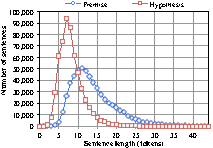
\includegraphics[width=3.05in]{length_dist}
    % From 1.0rc2, though still accurate as of rc3
\todo{Replace w/ mean+SD if low on space.}
\caption{\label{b-table}The distribution of sentence length.} 
\end{figure}

\begin{table}
\center
  %\setlength{\tabcolsep}{15pt}
  %\renewcommand{\arraystretch}{1.2}
  \begin{tabular}{l l} 
    \toprule
\multicolumn{2}{l}{\textbf{Data set sizes:}}\\
Training pairs &  550,152\\
Development pairs &  10,000\\
Test pairs & 10,000\\
\midrule
\multicolumn{2}{l}{\textbf{Sentence length:}}\\
Premise mean token count & 14.1\\
Hypothesis mean token count & 8.3 \\
\midrule
\multicolumn{2}{l}{\textbf{Parser output:}}\\
Premise `S'-rooted parses & 74.0\%\\
Hypothesis `S'-rooted parses & 88.9\%\\
Unique word tokens (ignoring case) & ...\\
    \bottomrule
  \end{tabular}
% From 1.0rc3
\todo{Unique word count.}
\caption{\label{collection-stats}Key statistics for the raw sentence pairs. Since the two halves of each pair were collected separately, we report some statistics for both.} 
\end{table}

\begin{table}
\center
  %\setlength{\tabcolsep}{15pt}
  %\renewcommand{\arraystretch}{1.2}
  \begin{tabular}{l l} 
    \toprule
\multicolumn{2}{l}{\textbf{General:}}\\
Validated pairs & 56,941\\
Pairs w/ unanimous gold label & 58.3\%\\
\midrule
\multicolumn{2}{l}{\textbf{Individual annotator label agreement:}}\\
Annotator label $=$ gold & 89.0\%\\
Annotator label $=$ author's label & 85.8\%\\
\midrule
\multicolumn{2}{l}{\textbf{Gold label/author's label agreement:}}\\
Gold label $=$ author's label & 91.2\%\\
Gold label $\ne$ author's label & 6.8\% \\
No gold label (no 3 labels match) & 2.0\%\\
\midrule
\multicolumn{2}{l}{\textbf{Fleiss $\kappa$:}}\\
    \ii{contradiction} & 0.77 \\
    \ii{entailment} & 0.72 \\
    \ii{neutral} & 0.60 \\
    Overall & 0.70 \\
    \bottomrule
  \end{tabular}
    % From 1.0rc3
\caption{\label{validation-stats}Key statistics for the validated pairs. The \ii{author's label} is the label that was used by the worker who wrote the premise to create the sentence pair. A \ii{gold label} reflects a consensus of three votes among the author and the four annotators.} 
\end{table}

\paragraph{Partition} We distribute the corpus with a pre-specified train/test/development split. The test and development sets contain 10k examples each. Each original ImageFlickr caption occurs in only one of the three sets, and all of the examples in the test and development sets have gone through validation.


\paragraph{Parses}

The distributed corpus includes parses for every sentence produced by the Stanford PCFG Parser \cite{klein2003accurate} (trained on the standard training set as well as on the Brown Corpus; \citealt{francis1979brown}), both in the standard PTB format and in the binarized unlabeled format used by tree-structured neural network models, as in \S\ref{sentence-embedding}.

\noindent\todo{Use version number for 4/20/15 model}

\paragraph{General evaluation standards}
While we hope that the corpus will be valuable in a variety of ways, we encourage researchers working on tools for semantic representation and inference to evaluate on our data in a uniform way: training on only the (parsed and/or unparsed) sentences included in the training set, and doing final evaluations on only the subset of the test set for which there are single gold labels.

\section{Our data as a platform for evaluation}

The most immediate application for our corpus is in developing models for the task of NLI. In particular, since it is dramatically larger than any existing corpus of comparable quality, we expect it to be suitable for training parameter-rich models like neural networks, which have not previously been competetive at this task. In this section, we explore the performance of a range of standard and novel models trained on the corpus.

\subsection{Standard entailment models}

The first class of models is from the Excitement Open
  Platform (EOP,
  \citealt{pado2014design,magnini2014excitement})---an open source platform for RTE research.
%  which
%  is distributed alongside a number of RTE pipelines.
We additionally evaluate against a strong but simple classifier-based model with
  both unlexicalized and lexicalized features.

%
% EOP
%
\paragraph{Excitement Open Platform}
% what is EOP
The Excitement Open Platform is a tool to quickly develop NLI systems
  while sharing components such as common lexical resources and 
  evaluation sets.
We evaluate against two algorithms included in the distribution:
%  and also evaluated in \newcite{magnini2014excitement}.
%These are: 
  a simple edit-distance based algorithm and
  a classifier-based algorithm.
%  (3) an algorithm based around tree transformations.

%% 9 systems compared against
%A number of systems have been built using the platform, 9 of them
%  applicable to English are publicly distributed with version 1.2.1
%  of the software.
%% these fall into 2 classes
%These fall into two classes of algorithms: 2 are edit distance based,
%  whereas the remaining 7 make use of different features in a
%  maximum entropy classifier.
%
%%% methodology
%%We convert the 3-way classification task in SNLI into the RTE setting
%%  by labeling both the \unknown\ and \contradiction\
%%  labels as negative entailment, and treating the \entailment\ label as
%%  the positive entailment.
%%This creates a biased dataset of 66\% negative examples.
%% we report the best results from each class
%We run the top performing edit-distance based algorithm and the top
%  performing classifier-based algorithm on our test set, as
%  determined by performance on the development set.
%Note that these models were run using the default configuration
%  with minimal tuning.
%The results should therefore be taken as a strong baseline for
%  NLI-style approaches to the problem, rather than necessarily
%  representing the state-of-the-art system's performance on the
%  task.
%%We run each of the 9 algorithms distributed with EOP on the 2-class
%%  SNLI dataset, and report results for the best edit distance 
%%  configuration and the best classifier based configuration, as
%%  determined by performance on the development set.

%
% EOP RESULTS TABLE
%

% The table
\begin{table}
\begin{center}
\def\t#1{\small{#1}}
\begin{tabular}{l@{\hskip \colspaceL}c@{\hskip \colspaceL}c@{\hskip \colspaceL}c}
\toprule
\b{System} & \b{SNLI} & \b{SICK} & \b{RTE-3} \\
\midrule
\t{Edit Distance Based}        & \t{71.9} & \t{65.4} & \b{61.9} \\
\t{Classifier Based}           & \b{72.2} & \b{71.4} & \t{61.5} \\
%\midrule
%\t{Classifier Based (3-class)} & \t{??.?} & \t{65.6} & \t{} \\
%\t{Transformation Based} & \t{36.0} & \t{76.7} & \t{56.4} \\  % broken! At least, on SNLI...
\bottomrule
\end{tabular}
\end{center}
% The caption
\caption{
\label{tab:eopresults}
2-class test accuracy for two systems included in the
  Excitement Open Platform.
%All RTE results are 2-class accuracy.
%The transformation-based model allows for 3-class predictions on our
%  corpus and SICK; these are reported in the last row.
}
\end{table}
%
% END EOP RESULTS TABLE
%

% the best systems
We report results in \reftab{tab:eopresults}, covering both our own test set,
  the SICK test data, and the standard RTE-3 test set \cite{giampiccolo2007third}.
Each of the models was trained on its own training set.
%The results for RTE-3 are taken from \newcite{magnini2014excitement}.
The edit distance and classifier based models are evaluated only on
  2-class entailment; all RTE results are likewise reported for 2-class entailment.
To convert 3-class problems like SICK and SNLI to this setting, all instances
  of \contradiction\ and \unknown\ are converted to nonentailment.
This yields a chance baseline accuracy of 66\% on SNLI, and 71\% on SICK.
We train these models without using any of the included lexical
  resources, so these results do not represent state-of-the-art
  RTE systems, but rather give an indication of the relative
  difficulties of the datasets.

%The best edit distance algorithm tunes the weight of the three 
%  case-insensitive edit distance operations on the training set, 
%  after removing stop words.
%The best classifier-based system makes use of information from
%  WordNet \cite{miller1995wordnet} and VerbOcean
%  \cite{chklovski2004verbocean}, and makes use of features
%  based on tree patterns and dependency tree skeletons
%  \cite{wang2007recognizing}.
%Unsurprisingly, the classification-based approach outperforms simple
%  edit distance metrics, and performs quite well despite relatively
%  little lexicalization.
%\todo{Is the RTE3 model trained on RTE3?}

%
% Lexicalized Classifier
%
\paragraph{Lexicalized Classifier}
Unlike the RTE datasets, SNLI's size supports approaches which make use of rich lexicalized features.
We evaluate a simple lexicalized classifier to explore the ability of non-specialized models to exploit these features in lieu of more involved language understanding.
Our classifier implements 6 feature types:
\begin{enumerate}
\setlength\itemsep{-0.25em}
  \item The BLEU score of the \hypothesis\ with respect
  to the \premise, using an n-gram length between 1 and 4.

  \item The length difference between the \hypothesis\ and the \premise, as a real-valued
  feature.

  \item The overlap between words in the \premise\ and \hypothesis,
  both as an absolute count and a percentage of possible overlap, and both over 
  all words and over just nouns, verbs, adjectives, 
  and adverbs.
  
  \item\label{lst:ngram} An indicator for every unigram and bigram in the \hypothesis.

  \item\label{lst:unigram} Cross-unigrams: for every pair of words across the \premise\ and \hypothesis\ which share a 
  POS tag, an indicator feature over the two words.
  
  \item\label{lst:bigram} Cross-bigrams: for every pair of bigrams across the \premise\ and \hypothesis\ which share a 
  POS tag on the second word, an indicator feature over the two bigrams.
\end{enumerate}

%
% BOW RESULTS TABLE
%

% The table
\begin{table}
\begin{center}
\begin{tabular}{l@{\hskip \colspaceL}c@{\hskip \colspaceS}c@{\hskip \colspaceL}c}
\toprule
\b{System}	 & \multicolumn{2}{c}{\hspace{-1.2em}\b{SNLI}} & \b{SICK}\\
 & \t{Train} & \t{Test} & \t{Test}\\
\midrule
\t{Lexicalized}            & \t{99.7}  & \b{78.2} & \b{77.3} \\ % & \t{78.7}
\t{Unigrams Only}          & \t{93.1} & \t{71.6} & \t{74.0} \\ % & \t{72.2}
\t{Unlexicalized}          & \t{49.4} & \t{50.4} & \t{69.4}\\ % & \t{50.1} % Last value was 50.39; rounded for consistency.
\bottomrule
\end{tabular}
\end{center}
% The caption
\caption{
\label{tab:bowresults}
3-class accuracy, training on either our data or SICK, including models lacking cross-bigram features 
  (Feature \ref{lst:bigram}), and lacking all lexical
  features (Features \ref{lst:ngram}--\ref{lst:bigram}). For the model trained on SNLI, we report results both on the test set and the training set to judge overfitting.
}
\end{table}
%
% END BOW RESULTS TABLE
%


% Results
We report results in \reftab{tab:bowresults}, along with ablation studies for removing
  the cross-bigram features (leaving only the cross-unigram feature)
  and for removing all lexicalized features.
% Insights 1: lexicalization helps a bunch
On our large corpus in particular, there is a substantial jump in accuracy from using
  lexicalized features, and another from using the very sparse
  cross-bigram features.
The latter  result can be explained if
  the classifier automatically learns to recognize explicit negations and adjective
  modification, and a similar result was shown in
  \newcite{sidaw12simple} for bigram features in sentiment analysis.
  
% Insight 2: do well without alignments
Another surprising fact is that the classifier performs as well as it
  does without any notion of alignment or tree transformations.
Although we expect that richer models would perform better,
  the results suggest that given enough data, cross bigrams with the noisy 
  part-of-speech overlap constraint can produce an effective model.

%In fact, the addition of these features alone allow the classifier to
%  outperform many of the .
%  This seems initially surprising, but it makes sense given how our corpus differs from existing ones:
%  the EOP systems have been tuned on relatively small corpora
%  ($\approx$1600 examples), whereas a classifier trained on our corpus can make use of
%  over two orders of magnitude more data.

\subsection{Sentence embeddings and NLI}\label{sentence-embedding}

SNLI is suitably large and diverse to make it possible to train neural network models that produce distributed representations of sentence meaning. In this section, we compare the performance of three such models on the corpus. To focus specifically on the strengths of these models at producing informative sentence representations, we use sentence embedding as an intermediate step in the NLI classification task: each model must produce a vector representation of each of the two sentences without using any context from the other sentence, and the two resulting vectors are then passed to a neural network classifier which predicts the label for the pair. This choice allows us to focus on existing models for sentence embedding, and it allows us to evaluate the ability of those models to learn useful representations of meaning (which may be independently useful for subsequent tasks), at the cost of excluding from consideration possible strong neural models for NLI that directly compare the two inputs at the word or phrase level.


\begin{figure}[tp]
  \centering
\scalebox{0.85}{
 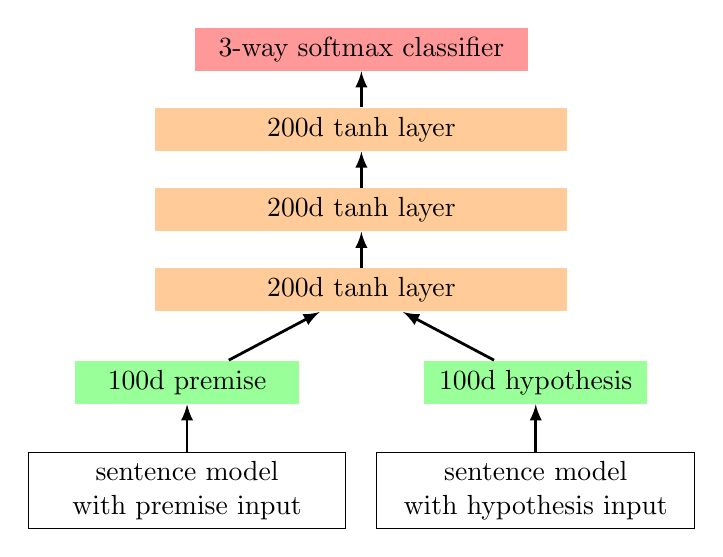
\begin{tikzpicture}
    \def\dx{21pt}
    \def\dy{29pt}

    \tikzstyle{label}=[text width=40mm,align=center]    
    \tikzstyle{softmax}=[fill=red!40,text width=40mm,align=center]
    \tikzstyle{preclass}=[fill=orange!40,text width=50mm,align=center]
    \tikzstyle{e}=[fill=green!40,text width=26mm,align=center]
    \tikzstyle{m}=[draw=black,text width=38mm,align=center]    
    
    \node[softmax]  (softmax) at (0*\dx,6*\dy) {3-way softmax classifier};
    \node[preclass]  (pc3) at (0*\dx,5*\dy) {200d $\tanh$ layer};
    \node[preclass]  (pc2) at (0*\dx,4*\dy) {200d $\tanh$ layer};
    \node[preclass]  (pc1) at (0*\dx,3*\dy) {200d $\tanh$ layer};
    \node[e]  (pe) at (-3*\dx,1.85*\dy) {100d premise};
    \node[e]  (he) at (3*\dx,1.85*\dy) {100d hypothesis};
    \node[m]  (pem) at (-3*\dx,0.5*\dy) {sentence model\\ with premise input};
    \node[m]  (hem) at (3*\dx,0.5*\dy) {sentence model\\ with hypothesis input};    
    
    \pgfsetarrowsend{latex}
    \tikzstyle{fwd} = [draw=black, line width=1pt]

          \draw [fwd] (pc3) -- (softmax);
          \draw [fwd] (pc2) -- (pc3);
          \draw [fwd] (pc1) -- (pc2);
          \draw [fwd] (pe) -- (pc1);
          \draw [fwd] (he) -- (pc1);
          \draw [fwd] (hem) -- (he);
          \draw [fwd] (pem) -- (pe);

  \end{tikzpicture}}
	
        \caption{The neural network classification architecture: for each sentence embedding model evaluated in \reftabs{tab:nnresults}{tab:transferresults}, two identical copies of the model are run with the two sentences as input, and their outputs are used as the two 100d inputs shown here.}
  \label{modelstructure}
\end{figure}

Our neural network classifier, depicted in \reffig{modelstructure} (and based on a one-layer model in \citealt{Bowman:Potts:Manning:2014}), is simply a stack of three 200d $\tanh$ layers, with the bottom layer taking the concatenated sentence representations as input and the top layer feeding a softmax classifier, all trained jointly with the sentence embedding model itself.

We test three sentence embedding models, each set to use 100d phrase and sentence embeddings. Our baseline sentence embedding model simply sums the embeddings of the words in each sentence. In addition, we experiment with two simple sequence embedding models: a plain RNN and an LSTM RNN \cite{hochreiter1997long}. Both use the simple conventional layout with one layer per input token.

The word embeddings for all of the models are initialized with the 300d reference GloVe vectors (840B token version, \citealt{pennington2014glove}) and fine-tuned as part of training. In addition, all of the models use an additional $\tanh$ neural network layer to map these 300d embeddings into the lower-dimensional phrase and sentence embedding space. All of the models are randomly initialized using standard techniques and trained using AdaDelta \cite{zeiler2012adadelta} minibatch SGD until performance on the development set stops improving. We applied L2 regularization to all models, manually tuning the strength coefficient $\lambda$ for each, and additionally applied dropout \cite{srivastava2014dropout} to the inputs and outputs of the sentence embedding models (though not to its internal connections) with a fixed dropout rate. All models were implemented in a common framework for this paper, and the implementations will be made available at publication time.

\begin{table}
\begin{center}
\begin{tabular}{l@{\hskip \colspaceL}@{\hskip \colspaceL}c@{\hskip \colspaceL}c}
\toprule
\textbf{Sentence model} & \b{Train}  & \b{Test}\\
\midrule
\t{100d Sum of words}            & \t{79.3} & \t{75.3} \\
% scr/snlirc3d-snlirc3-only-l0.0001-dim100-ed300-td3-pen200-do0.9-0.9-co3-comp-1-dp1-gc5-lstminit5/stat_log
% 290500, dev 76.4, converged

\t{100d RNN}            & \t{73.1} & \t{72.2} \\	
% scr/snlirc3d-snlirc3-only-l0.0001-dim100-ed300-td3-pen200-do0.9-0.9-co3-comp3-dp1-gc5-lstminit5/stat_log
% 338500, dev 72.5, mostly converged

\t{100d LSTM RNN}            & \t{84.8} & \b{77.6} \\
% scr/snlirc3d-snlirc3-only-l3e-05-dim100-ed300-td3-pen200-do0.95-0.95-co3-comp2-dp1-gc5-lstminit5/stat_log
% 372000, dev 79.11, mostly converged

% \t{100d TreeRNN}            & \t{69?} & \t{69?} \\
% \t{50d TreeRNTN}            & \t{61?} & \t{60?} \\
% \t{100d LSTM TreeRNN}            & \t{72?} & \t{73?} \\
\bottomrule
\end{tabular}
\end{center}
% The caption
\caption{
\label{tab:nnresults}
Accuracy in 3-class classification on our training and test sets for each model.
}
\end{table}

The results are shown in \reftab{tab:nnresults}. The sum of words model performed slightly worse than the fundamentally similar lexicalized classifier---while the sum of words model is able to use pretrained word embeddings to better handle rare words, it lacks even the rudimentary sensitivity to word order that the lexicalized model's bigram features provide. Of the two RNN models, the LSTM's more robust ability to learn long-term dependencies serves it well, giving it a substantial advantage over the plain RNN, and  resulting in performance that is essentially equivalent to the lexicalized classifier on the test set (LSTM performance near the stopping iteration varies by up to 0.5\% between evaluation steps). While the lexicalized model fits the test set perfectly, the gap between train and test set accuracy is relatively small for all three neural network models, suggesting that research into significantly higher capacity versions of these models could be productive.

\subsection{Analysis and discussion}

\Reffig{fig:bowlearncurve} shows a learning curve for the LSTM and the lexicalized and unlexicalized feature-based models. This learning curve shows that the large size of the corpus is crucial to both the LSTM and the lexicalized model, and suggests that additional data would yield still better performance for both. In addition, though the LSTM and the lexicalized model show similar performance when trained on the current full corpus, the somewhat steeper slope for the LSTM hints that its ability to learn arbitrarily structured representations of sentence meaning may give it an advantage over the more constrained lexicalized model on still larger datasets.

% useful resource in the development of more sophisticated SE models

\Fig{learning_curves_bow.pdf}{0.45}{bowlearncurve}{
A learning curve for the lexicalized and unlexicalized baseline classifiers and the LSTM,
plotted on a log scale. The y-axis starts at a random-chance accuracy of 33\%. The minibatch size of 64 that we used to tune the LSTM sets a lower bound on data for that model.}

% Insights 2: the learning curve for the unlexicalized classifier is sad
We were struck by the speed with which the lexicalized classifier outperforms its unlexicalized counterpart.
With only 100 training examples, the cross-bigram classifier is already performing better.
Empirically, we find that the top weighted features for the classifier
  trained on 100 examples tend to be high precision entailments;
  e.g.,
  \textit{playing} $\rightarrow$ \textit{outside}
  (most scenes are outdoors), \textit{a banana} $\rightarrow$
  \textit{person eating}.
If relatively few spurious entailments get high weight---as it appears
is the case---then it makes sense that, when these do fire, they
boost accuracy in identifying entailments.
  
There are revealing patterns in the errors common to all the models
considered here. Despite the large size of the training corpus and the
distributional information captured by GloVe initialization, many
lexical relationships are still misanalyzed, leading to incorrect
predictions of \ii{independent}, even for pairs that are common in the
training corpus like \word{beach}/\word{surf} and
\word{sprinter}/\word{runner}. Semantic mistakes at the phrasal level
(e.g., predicting contradiction for \word{A male is placing an order in a 
deli}/\word{A man buying a sandwich at a deli}) indicate
that additional attention to compositional semantics would pay off.
%
% Others that could replace the above:
% \word{Two teen girls relax on a black futon}/\word{Two young girls are sitting inside}
% \word{A male is placing an order in a deli}/\word{A man buying a sandwich at a deli}
% \word{A shopper buys cat food at a Walmart}/\word{A person shops for their pet at a store}
However, many of the persistent problems run deeper, to inferences
that depend on world knowledge and context-specific inferences, as in
the entailment pair \word{A race car driver leaps from a burning
  car}/\word{A race car driver escaping danger}, for which both
the lexicalized classifier and the LSTM predict \ii{neutral}. 
In other cases, the models' attempts to shortcut this kind of inference 
through lexical cues can lead them astray. 
Some of these examples have qualities
reminiscent of Winograd schemas \cite{Winograd:1972,Levesque:2013}. For
example, all the models wrongly predict
entailment for \word{A young girl throws sand toward the
  ocean}/\word{A girl can't stand the ocean}, presumably because of
distributional associations between \word{throws} and \word{can't
  stand}.

Analysis of the models' predictions also yields insights into the
extent to which they grapple with event and entity coreference. For
the most part, the original image prompts contained a focal element
that the caption writer identified with a syntactic subject, following
information structuring conventions associating subjects and topics in
English \cite{Ward04}. Our annotators generally followed suit, writing
sentences that, while structurally diverse, share topic/focus (theme/rheme)
structure with their premises.
This promotes a coherent, situation-specific construal of each sentence
pair. This is information that our models can easily take advantage
of, but it can lead them astray. For instance, all of them stumble
with the amusingly simple case \emph{A woman prepares ingredients for
  a bowl of soup}/\emph{A soup bowl prepares a woman}, in which prior
expectations about parallelism are not met. Another headline example
of this type is \emph{A man wearing padded arm protection is being
  bitten by a German shepherd dog}/\emph{A man bit a dog}, which all
the models wrongly diagnose as \ii{entailment}, though the sentences
report two very different stories.

\section{Transfer learning with SICK}

To the extent that successfully training a neural network model like our LSTM on SNLI forces that model to encode broadly accurate representations of English scene descriptions and to build an entailment classifier over those relations, we should expect it to be readily possible to adapt the trained model for use on other NLI tasks. In this section, we evaluate on the SICK entailment task using a simple transfer learning method and achieve competitive results.

\begin{table}
\begin{center}
\begin{tabular}{l@{\hskip \colspaceL}@{\hskip \colspaceL}c@{\hskip \colspaceL}c}
\toprule
\textbf{Training sets} & \b{Train}  & \b{Test}\\
\midrule
\t{Our data only}            & \t{42.0} & \t{46.7} \\
% scr/transfer5-sick-only-transfer-l0.0001-dim100-ed300-td3-pen200-do0.95-0.95-ws3-adi1-comp2-cdim1/stat_log
% Step 0, no learning intended after transfer
\t{SICK only}            & \t{100} & \t{71.3} \\
% From: ~/quant/transfer-sick-only-l0.0001-dim50-ed200-td3-pen100-do0.9-0.9-ws1-par0-comp2-cdim1/
\t{Our data and SICK (transfer)}            & \t{99.9} & \b{80.8} \\
% From: ~/quant/transfer5-sick-only-transfer-l0.0001-dim100-ed300-td3-pen200-do0.95-0.95-ws3-adi0-comp2-cdim1/stat_log
\bottomrule
\end{tabular}
\end{center}

\caption{\label{tab:transferresults}
LSTM 3-class accuracy on the SICK train and test sets under three training regimes.} 
% TODO (Gabor): Report training accuracy for the model trained on SICK.
\end{table}


To perform transfer, we take the parameters of the LSTM RNN model trained on SNLI and use them to initialize a new model, which is trained from that point only on the training portion of SICK. The only newly initialized parameters are softmax layer parameters and the embeddings for words that appear in SICK, but not in SNLI (which are populated with GloVe embeddings as above). We use the same model hyperparameters that were used to train the original model, with the exception of the L2 regularization strength, which is re-tuned. We additionally transfer the accumulators that are used by AdaDelta to set the learning rates. This lowers the starting learning rates, and is intended to ensure that the model does not learn too quickly in its first few epochs after transfer and destroy the knowledge accumulated in the pre-transfer phase of training. We tune the regularization parameter separately for each case. 

The results are shown in \reftab{tab:transferresults}. Training on SICK alone yields poor performance, and the model trained on SNLI fails when tested on SICK data, labeling more \ii{neutral} examples as \ii{contradiction}s than correctly, possibly as a result of subtle differences in the label definitions. Transferring representations, in contrast, yields the best performance yet reported on SICK for an unaugmented neural network model, surpasses the available EOP models, and approaches both the overall state of the art at 84.6\% \cite{lai2014illinois} and the 84\% level of interannotator agreement, which likely represents an approximate performance ceiling. This suggests that the introduction of a large high-quality corpus makes it  possible to train representation-learning models for sentence meaning that are competitive with the best hand-engineered models on inference tasks.

We attempted to apply this same transfer evaluation technique to the RTE-3 challenge, but found that the small training set (800 examples) did not allow the model to adapt to the unfamiliar genre of text used in that corpus, such that no training configuration yielded competitive performance.
Further research on effective transfer learning on small data sets with neural models might facilitate improvements here.


% A woman prepares ingredients for a bowl of soup.	A soup bowl prepares a woman.


\section{SNLI and transfer learning}\label{sec:transfer}

We argue that for a sentence representation to provide the information necessary to reliably perform NLI classification, it must contain a faithful and thorough description of the sentence's meaning. This claim has a readily testable consequence: the knowledge that a representation learning system learns when it is trained on SNLI should transfer well to any other task that involves understanding sentence meaning. To test this, we perform transfer learning experiments on four other tasks, in which models are initialized using the parameters of an LSTM RNN-based model trained on  on SNLI (as in \S\ref{sentence-embedding}) and then trained to convergence on the target tasks. 

We first evaluate on SICK (\citealt{marelli2014sick}), the smaller entailment corpus SNLI was modeled on, training on the standard 4.5k training sentence pairs. We then evaluate on SUBJ (\citealt{pang2004sentimental}), a two-way sentence classification task, using 5-fold cross-validation over the 10k sentences. We next evaluate on the SST (\citealt{socher2013acl1}), a five-way sentiment classification task with labels for both phrases and sentences. We train on both types of label within the 8.5k sentence training set and test on only the sentence-level labels in the test set. We finally evaluate on PragBank, an 800 example 6-way sentence classification task focused on veridicality. \todo{Cite} ....

We use pretrained parameters for all of the LSTM parameters, pretrained parameters for the $\tanh$ layers in the classifier stack, and pretrained embeddings for all of the words that occurred in both corpora, randomly initializing only the softmax layer and the remaining word embeddings. In order to use this starategy in sentence classification tasks, we pass the classifier the embedding of the sentence to be classified in the hypothesis input position, as well as a zero vector in the premise input position. After transfer, we re-initialize the accumulators in AdaDelta to re-set the learning rates to high values. We additionally use L2 regularization with each task, separately tuning the regularization strength on the transfer model and the corresponding baseline model without transfer.

\todo{Do we still want to re-initialize LRs?}
\todo{Do we want to use all four target tasks?}

\begin{table}
\begin{center}
\begin{tabular}{l@{\hskip \colspaceL}c@{\hskip \colspaceS}c@{\hskip \colspaceS}c@{\hskip \colspaceS}c@{\hskip \colspaceS}c}
\hline
\textbf{Corpus} & \multicolumn{2}{c}{\b{Train Acc.}} &\multicolumn{3}{c}{ \b{Test Acc.}} \\
 & \t{cold start} & \t{transfer} & \t{cold start} & \t{transfer} & \t{SotA} \\
\hline
\t{SICK}            & \t{98} & \t{95} & \t{63?} & \t{80.0?} & \t{84.5} \\
\t{SUBJ}          & \t{??.?} & \t{??.?} & \t{??.?} & \t{??.?}& \t{??.?} \\
\t{SST}          & \t{??.?} & \t{??.?} & \t{43?} & \t{43?} & \t{50.6}\\
\t{PragBank}          & \t{??.?} & \t{??.?} & \t{??.?} & \t{??.?}& \t{??.?} \\
\hline
\end{tabular}
\end{center}

\caption{\label{tab:transferresults}
The performance of an LSTM RNN model on four tasks under both a random initialization and a transfer initialization copied from a model trained on SNLI. All figures are classification accuracy, except for PragBank, where report macroaveraged F1 to enable comparison with existing results on that task. \todo{Final numbers.}} 

\end{table}

The final column shows the state of the art results from \cite{lai2014illinois}, TODO, \cite{tai2015improved}, TODO, respectively.
\todo{Does Tai have the SotA on SST?}

The results are shown in Table~\ref{tab:transferresults}. For each task, the transfer model is compared with a model that was initialized randomly as normal. Note that \todo{something interesting happens}. Within the domain of NLI, our transfer model shows the best number yet reported on SICK for a fully-learned model, and approaches the overall state of the art (and to the 84\% level of interannotator agreement, a likely performance cieling), while the randomly initialized model performs poorly. This suggests that the introduction of SNLI makes it newly possible to train representation learning models for sentence meaning of a level of quality that is competitive with the best hand-engineered models on semantically sophisticated tasks.

\todo{something about the state of the art on the other tasks.}

\subsection{Conclusion}

\subsubsection*{Acknowledgments}

%
This work was supported in part by a Google Faculty Research Award,
NSF grant no.~IIS 1159679, % CP`
ONR grant no. N00014-10-1-0109, % CP
\todo{(CM: Any more?)}.
%
Any opinions, findings, and conclusions or recommendations expressed
in this material are those of the authors and do not necessarily
reflect the views of the NSF, ONR, \todo{\ldots}, or the US
government.

%%%

% \section*{Acknowledgments}

% Do not number the acknowledgment section.

\bibliographystyle{acl}
\noindent\todo{Consistently use first initials in bib.}
\noindent\todo{Anonymize SNLI to something non-'Stanford'}
\bibliography{MLSemantics} 

\end{document}
